% https://books.google.com.co/books?id=m3QTSMYm5rkC&printsec=frontcover
% https://books.google.com.co/books?id=QxdNBQAAQBAJ&lpg=PA52&hl=es&pg=PP1#v=onepage&q&f=false
% https://oeis.org/wiki/List_of_LaTeX_mathematical_symbols
% https://www.overleaf.com/learn/latex/Mathematical_expressions
% http://www.unipamplona.edu.co/unipamplona/portalIG/home_23/recursos/general/11072012/grafo3.pdf
% https://www.geeksforgeeks.org/difference-between-deterministic-and-non-deterministic-algorithms/
% http://www.personal.kent.edu/~rmuhamma/GraphTheory/MyGraphTheory/defEx.htm
% http://data-mining.philippe-fournier-viger.com/introduction-frequent-subgraph-mining/
% http://www.analytictech.com/networks/graphtheory.htm
% https://es.wikipedia.org/wiki/Grafo_conexo
% https://martin-thoma.com/how-to-visualize-graph-algorithms-with-latex/

\section{Teoría de grafos}\label{graph theory}
En matemáticas y en ciencias de la computación, la teoría de grafos estudia las propiedades de los grafos. Un grafo \( G(V,E) \) es una colección de puntos, llamados vértices o nodos \( V = \{ v_1, v_2, \dots \} \), y segmentos de línea que conectan esos puntos, llamados aristas o arcos (en inglés \textit{edges}) \( E = \{ e_1, e_2, \dots \} \); cada arista \( e \) tiene dos \textit{\gls{endpoints}}, que son vértices. Se escribe \( u \overset{e}{-} v \), y significa que la arista \( e \) incide sobre los vértices \( u \) y \( v \); en este caso se puede decir que \( e \) conecta los vértices \( u \) y \( v \), o que los vértices \( u \) y \( v \) son \gls{adjacents} \cite{even2011graph}.

\begin{figure}[H]
	\centering
	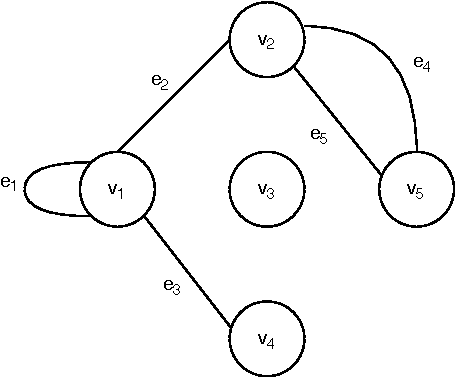
\includegraphics[width=0.35\linewidth]{document/GraphTheory/images/example-of-a-graph}
	\caption{Ejemplo de un grafo. \cite{even2011graph}}
	\label{fig:example-of-a-graph}
\end{figure}

\subsection{Grafo conexo}
Un grafo \( G \) es conexo, si por cada dos vértices \( u \) y \( v \), hay un camino (finito) que comienza en \( u \) y termina en \( v \) \cite{even2011graph}. Para verificar si un grafo \( G \) es conexo, se puede aplicar un \gls{deterministic algorithm} habitual, búsqueda en anchura en inglés \acrfull{bfs} o búsqueda en profundidad en inglés \acrfull{dfs}.

\begin{figure}[H]
	\centering
	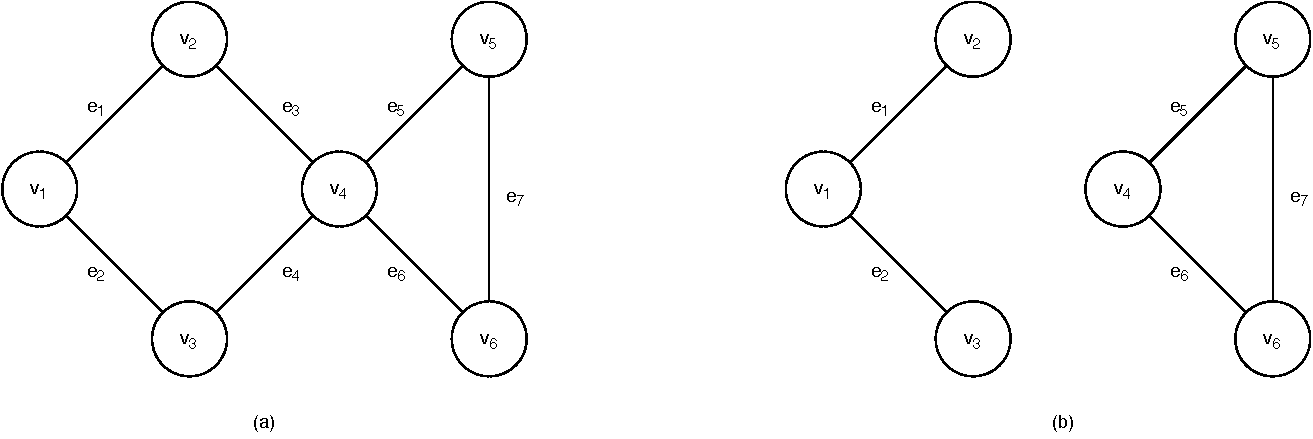
\includegraphics[width=1\linewidth]{document/GraphTheory/images/connected-disconnected-graph}
	\caption{Tipos de grafos. (a) Conexo. (b) Disconexo.}
	\label{fig:connected-disconnected-graph}
\end{figure}

% https://personales.unican.es/corcuerp/progcomp/slides/grafos.pdf
\subsection{Grafo dirigido o digrafo}
Un digrafo o grafo dirigido \( G(V,E) \) se define de manera similar a un grafo, excepto que el par de \textit{\gls{endpoints}} \( (u, v) \) de cada arista ahora está ordenado. Se escribe \( u \xrightarrow{\text{e}} v \), dónde \( u \) es el vértice inicial de \( e \); y \( v \) es el vértice final de \( e \). Se dice que la arista \( e \) está dirigida de \( u \) a \( v \) \cite{even2011graph}.

\begin{figure}[H]
	\centering
	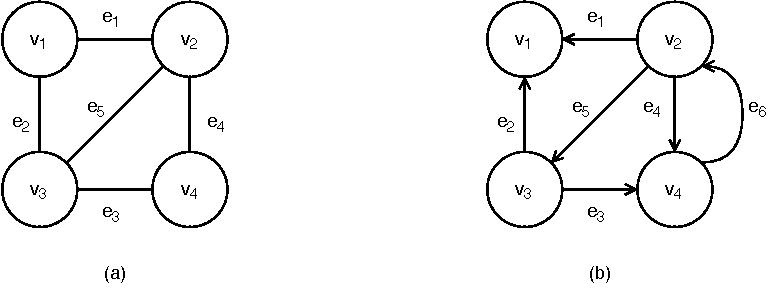
\includegraphics[width=0.6\linewidth]{document/GraphTheory/images/directed-undirected-graph}
	\caption{Tipos de grafos. (a) No dirigido. (b) Dirigido o digrafo. }
	\label{fig:directed-undirected-graph}
\end{figure}